\begin{center}
\underline{\Large{T.P.N°4: Tirantes de Hormigón Armado}}
\end{center}

\begin{enumerate}
\item Diseñar el tirante de ochava de la Figura \ref{figura1}, estimando la deformación elástica inicial del mismo para la condición considerada como más factible de servicio constituida por la totalidad de la carga permanente más el 50\% de la sobrecarga. Dibujar la sección.

\begin{figure}[H]
\begin{center}
	 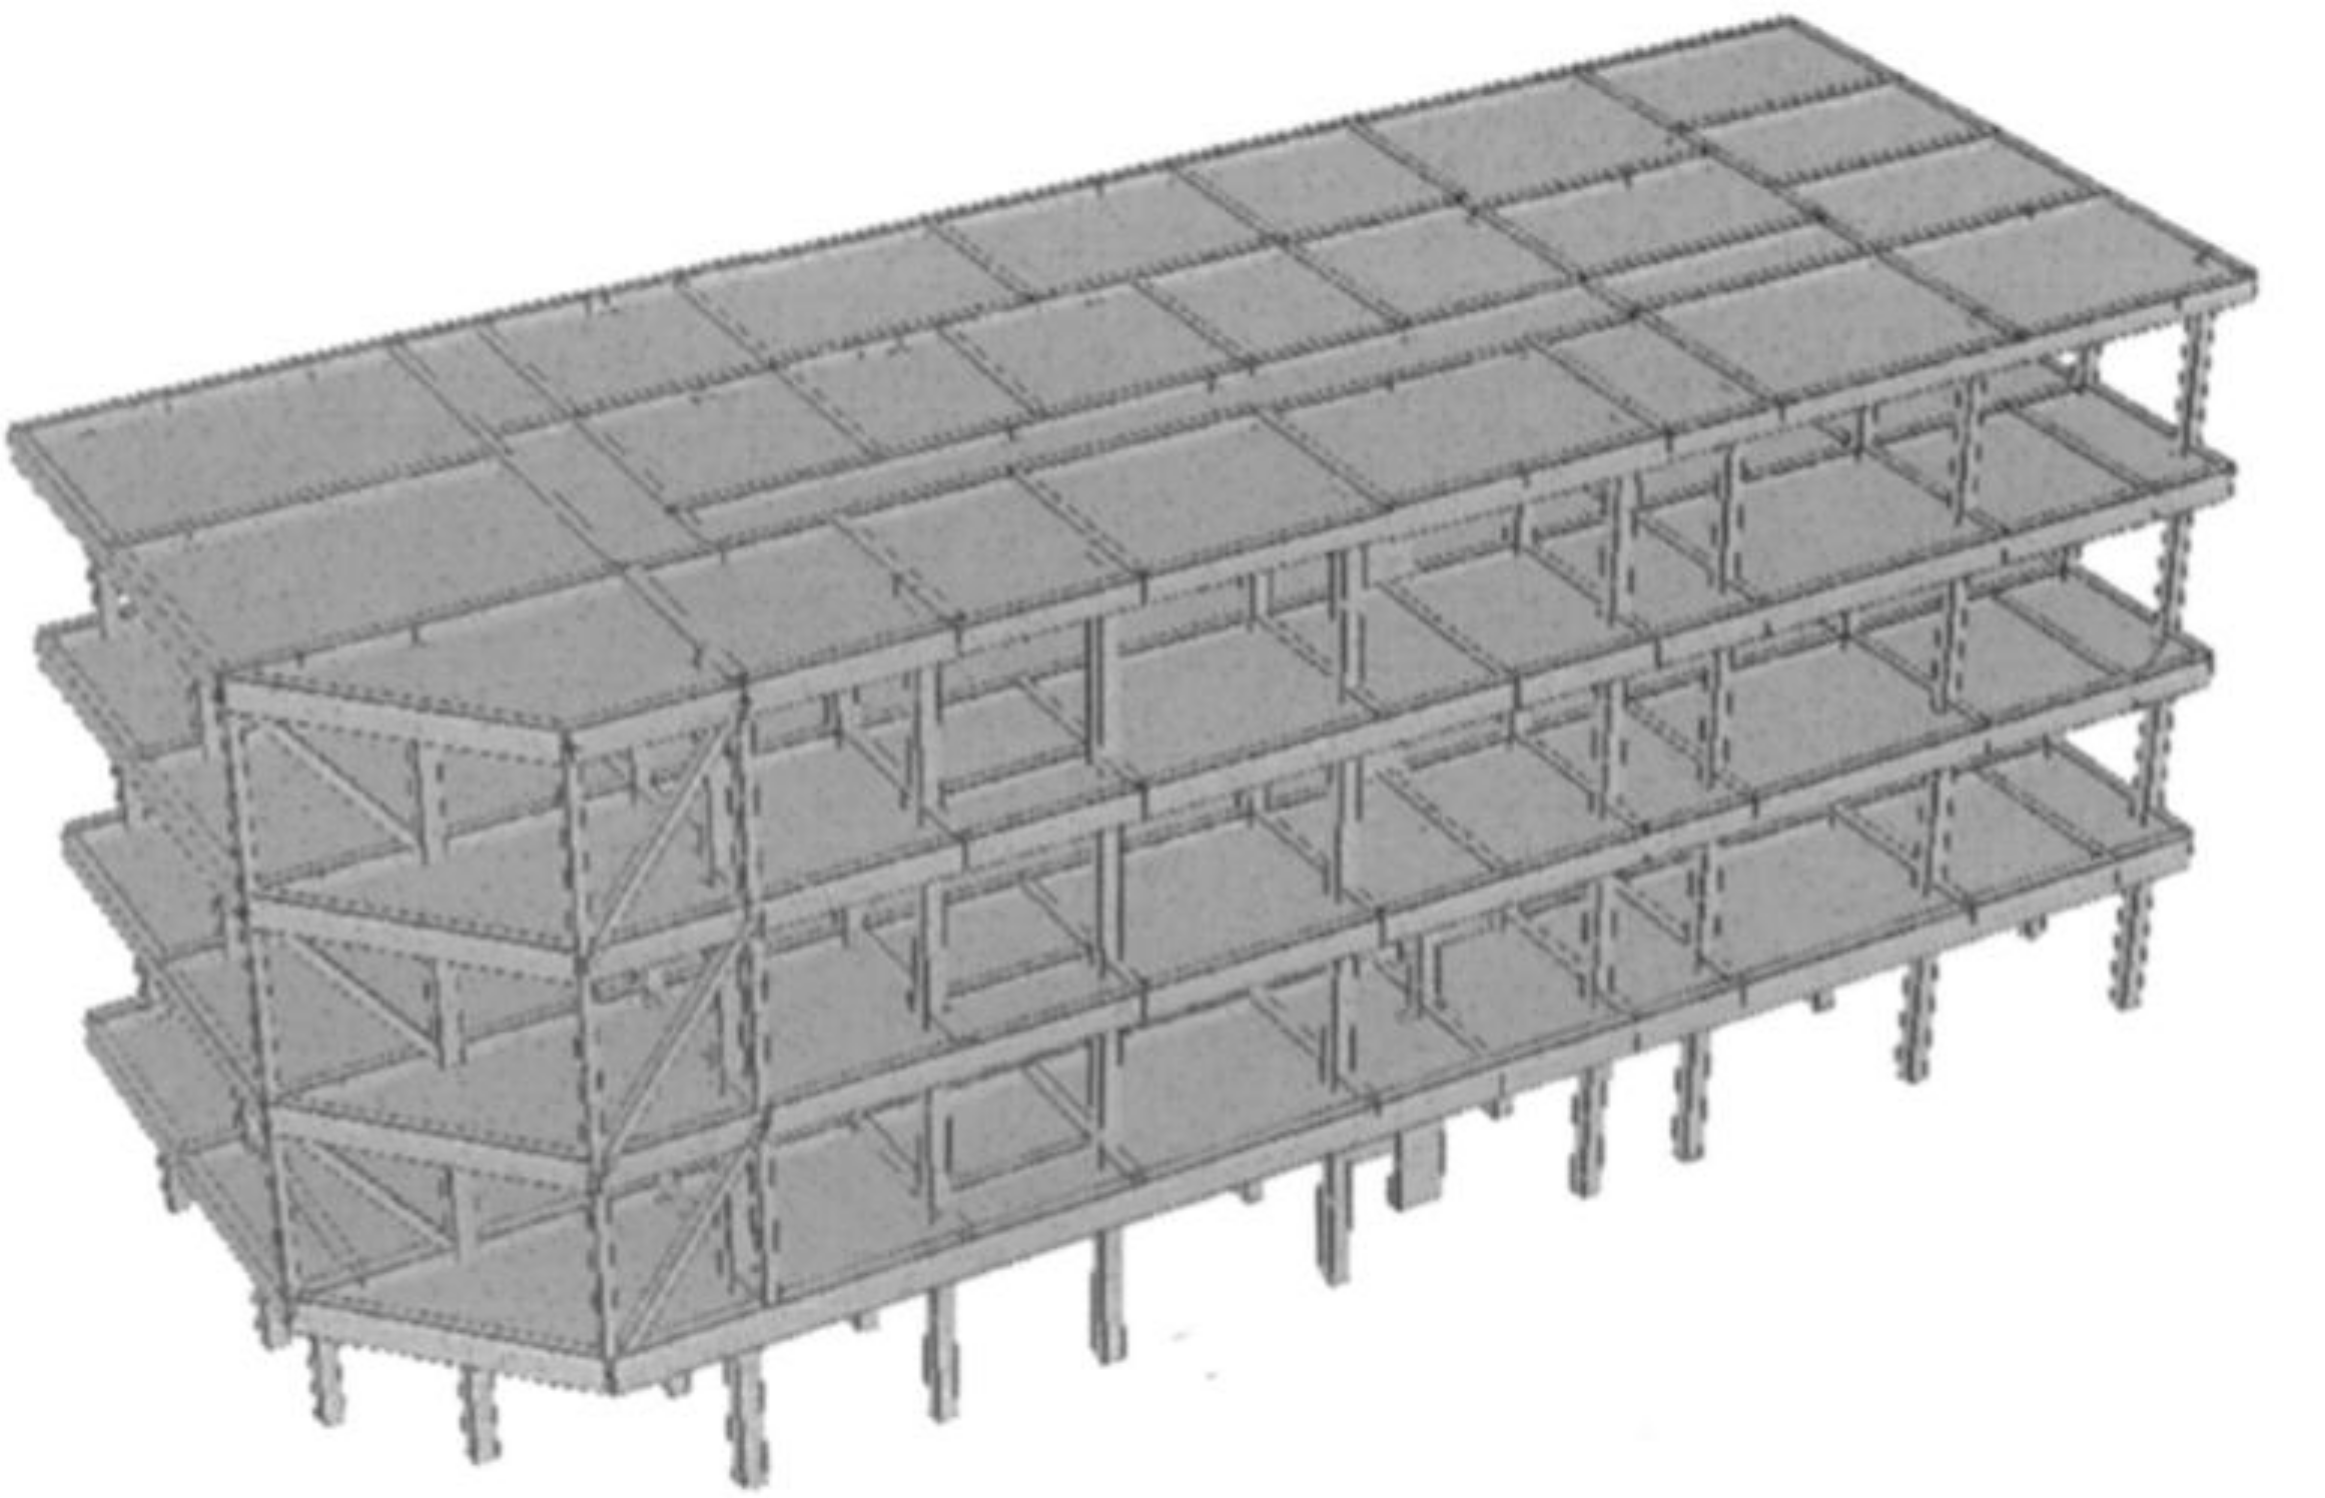
\includegraphics[scale = 0.9]{chapters/chapter_1/images/figura1.png}
     \caption{Esquema del edificio correspondiente al tensor del ejercicio 1}
     \label{figura1}
\end{center}
\end{figure}

\end{enumerate}

\begin{center}
\underline{\Large{Solución}}
\end{center}

\begin{enumerate}
\item \underline{Diseñar el tirante de ochava de la Figura 1}

\underline{Datos:}\\
Hormigón H-25 $\Rightarrow f'c = 250 \frac{Kg}{cm^2} = 25 MPa$\\
Acero ADN 42/50 $\Rightarrow fy = 4200 \frac{Kg}{cm^2} = 420 MPa$\\
b = h = 25cm\\
Recubrimiento Cc = 3cm\\
Estribos $\phi$ 8mm cada 15cm\\
Largo = 350cm\\
$P_D = 6.5t$\\
$P_L = 2.5t$\\

\begin{itemize}
\item \underline{Estado de cargas}

\begin{align*}
& P_{u1} = 1.4 \cdot P_D = 1.4 \cdot 6.5 t = \framebox{$9.1t$}\\
& P_{u2} = 1.2 \cdot P_D + 1.6 \cdot P_L = 1.2 \cdot 6.5 t + 1.6 \cdot 2.5 t = \framebox{$11.8t$}\\
& P_n = \frac{P_u}{\phi} = \frac{11.8 t}{0.9} = \framebox{$13.11t$}\\
& P_{servicio} = D + L = 6.5t + 2.5t = \framebox{$9t$}\\
& P_{permanente} = 6.5t + 0.5 \cdot 2.5t = \framebox{$7.75t$}
\end{align*}

\item \underline{Armadura por condición de rotura}

\begin{align*}
& A_s = \frac{P_n}{fy} = \frac{13110 Kg}{4200 \frac{Kg}{cm^2}} = \framebox{$3.12 cm^2$}
\end{align*}

\item \underline{Armadura por condición de ductilidad}

\begin{align*}
& \rho \geq \frac{A_s}{A_g} \geq \frac{\sqrt{f'c}}{1.8 \cdot fy} = \frac{\sqrt{25MPa}}{1.8 \cdot 420MPa} \Rightarrow \rho \geq 6.6 \cdot 10^{-3}\\
& A_s = \rho \cdot A_g = 6.6 \cdot 10^{-3} \cdot (25cm)^2 = \framebox{$4.13 cm^2$}
\end{align*}

Por lo tanto se diseña por condición de ductilidad.\\
El área necesaria es $\Rightarrow A_s = 4.13 cm^2 \Rightarrow$ Adopto 4 $\phi$ 12mm con $4.52 cm^2$ totales.\\

\item \underline{Verificación a la fisuración}

\begin{align*}
& dc = Cc + dbe + \frac{db}{2} = 3cm + 0.8cm + \frac{1.2cm}{2} = \framebox{$4.4 cm$}\\
& A = \frac{A_g}{\text{n° de barras}} = \frac{(250mm)^2}{4} = \framebox{$15625 mm^2$}\\
& f_{servicio}= \frac{P_{servicio}}{A_{s \text{ adoptada}}} = \frac{9000Kg}{4.52 cm^2} = 1991 \frac{Kg}{cm^2} = \framebox{$199 MPa$}\\
& \beta = 1 \text{ para tensores}\\
& W_k = \frac{1}{90000} \cdot \beta \cdot f_{servicio} \cdot \sqrt[3]{dc \cdot A}\\
& W_k = \frac{1}{90000} \cdot 1 \cdot 199MPa \cdot \sqrt[3]{44mm \cdot 15625 mm^2} = \framebox{$0.19 mm$}\\
& W_k < 0.30 mm\\
& 0.19mm < 0.30mm \quad \text{Verifica} \quad \surd
\end{align*}

\newpage
\item \underline{Verificación de deformación}

\begin{align*}
& E_c = 4700 \cdot \sqrt{f'c} = 4700 \cdot \sqrt{25MPa} = \framebox{$23500 MPa$}\\
& n = \frac{E_s}{E_c} = \frac{200000MPa}{23500MPa} = \framebox{8.51}\\
& A_{CR} = n \cdot A_s = 8.51 \cdot 4.52 cm^2 = \framebox{$38.46 cm^2$}\\
& A_{CH} = A_c + A_{CR} = (25cm)^2 + 38.46cm^2 = \framebox{$663.5 cm^2$}\\
& f't = \frac{\sqrt{f'c}}{3} = \frac{\sqrt{25MPa}}{3} = 1.66 MPa = \framebox{$16.6 \frac{Kg}{cm^2}$}\\
& P_{CR} = A_{CH} \cdot f't = 663.5 cm^2 \cdot 16.6 \frac{Kg}{cm^2} = \framebox{$11014 Kg$}\\
& A_{ef} = A_{CH} \cdot \Bigg(\frac{P_{CR}}{P_p} \Bigg)^3 + A_{CR} \cdot \Bigg[1-\Bigg(\frac{P_{CR}}{P_p} \Bigg)^3 \Bigg] \leq A_g\\
& A_{ef} = 663.5 cm^2 \cdot \Bigg(\frac{11014Kg}{7750Kg} \Bigg)^3 + 38.46 cm^2 \cdot \Bigg[1-\Bigg(\frac{11014Kg}{7750Kg} \Bigg)^3 \Bigg] \leq A_g\\
& A_{ef} = 1832 cm^2 > 625 cm^2 \Rightarrow \text{No se fisura}\\
& \varepsilon = \frac{P_p}{E_c \cdot A_{ef}} = \frac{7750Kg}{235000 \frac{Kg}{cm^2} \cdot 625 cm^2} = 5.2 \cdot 10^{-5}\\
& \Delta L = \varepsilon \cdot L < \Delta L_{admisible}\\
& \Delta L = \varepsilon \cdot L < \frac{L}{480}\\
& 5.2 \cdot 10^{-5} \cdot 3500mm < \frac{3500mm}{480}\\
& 0.18mm < 7.29mm \Rightarrow \text{Verifica} \quad \surd
\end{align*}

\end{itemize}
\end{enumerate}